\documentclass[10pt]{article}

\usepackage[margin=1in]{geometry} 
\usepackage{amsmath,amsthm,amssymb,bbm,subfig,graphicx,float,physics,listings,fontspec,color}
\usepackage{empheq}
\usepackage{titlesec}
\newfontfamily\Consolas{Consolas}
\definecolor{grey}{rgb}{0.9,0.9,0.9}
\lstset{basicstyle=\ttfamily, breaklines=true, numbers=left, numberstyle=\ttfamily, backgroundcolor=\color{grey}\ttfamily, keywordstyle=\color{blue}\ttfamily, stringstyle=\color{red}\ttfamily, commentstyle=\color{green}\ttfamily}
\DeclareMathOperator*{\argmin}{arg\,min}
\DeclareMathOperator*{\argmax}{arg\,max}
\DeclareMathOperator*{\vari}{var}

\begin{document}


% --------------------------------------------------------------
%                         Start here
% --------------------------------------------------------------
 
%\renewcommand{\qedsymbol}{\filledbox}
 
\title{\textbf{Report on Project 2}}%replace X with the appropriate number
\author{Zhunxuan Wang, 13300180086\\ %replace with your name
School of Mathematical Sciences} %if necessary, replace with your course title

\maketitle
\section{Logistic Regression}
\subsection{Bayes' Rule}
Based on the Bayes' theorem,
$$\Pr\left(y = 1 \mid \mathbf{x}\right) = \dfrac{p\left(\mathbf{x} \mid y = 1\right)\Pr\left(y = 1\right)}{p\left(\mathbf{x} \mid y = 1\right)\Pr\left(y = 1\right) + p\left(\mathbf{x} \mid y = 0\right)\Pr\left(y = 0\right)} = \dfrac{\alpha\,p\left(\mathbf{x} \mid y = 1\right)}{\alpha\,p\left(\mathbf{x} \mid y = 1\right) + \left(1 - \alpha\right)p\left(\mathbf{x} \mid y = 0\right)}\text{,}$$
and all the components of $\mathbf{x}$ are conditionally independent given $y$, thus
\begin{equation}
\begin{split}
\Pr\left(y = 1 \mid \mathbf{x}\right) &= \dfrac{\alpha\prod\limits_{i=1}^Dp\left(x_i \mid y = 1\right)}{\alpha\prod\limits_{i=1}^Dp\left(x_i \mid y = 1\right) + \left(1 - \alpha\right)\prod\limits_{i=1}^Dp\left(x_i \mid y = 0\right)}\\
&= \dfrac{\alpha\prod\limits_{i=1}^D\dfrac1{\sqrt{2\pi\sigma_i^2}}\exp-\dfrac{\left(x_i - \mu_{i1}\right)^2}{2\sigma_i^2}}{\alpha\prod\limits_{i=1}^D\dfrac1{\sqrt{2\pi\sigma_i^2}}\exp-\dfrac{\left(x_i - \mu_{i1}\right)^2}{2\sigma_i^2} + \left(1 - \alpha\right)\prod\limits_{i=1}^D\dfrac1{\sqrt{2\pi\sigma_i^2}}\exp-\dfrac{\left(x_i - \mu_{i0}\right)^2}{2\sigma_i^2}}\text{.}
\end{split}
\end{equation}
Dividing the numerator and denominator by the numerator, we have
\begin{equation}
\begin{split}
\Pr\left(y = 1 \mid \mathbf{x}\right) &= \dfrac{1}{1 + \dfrac{1 - \alpha}{\alpha}\exp\left[-\sum\limits_{i=1}^D\dfrac{\left(x_i - \mu_{i0}\right)^2 - \left(x_i - \mu_{i1}\right)^2}{2\sigma_i^2}\right]}\\
&= \dfrac{1}{1 + \dfrac{1 - \alpha}{\alpha}\exp\left[-\sum\limits_{i=1}^D\dfrac{\mu_{i1} - \mu_{i0}}{\sigma_i^2}\cdot x_i - \sum\limits_{i=1}^D\dfrac{\mu_{i0}^2 - \mu_{i1}^2}{2\sigma_i^2}\right]}\text{.}
\end{split}
\end{equation}
Reforming the formula above, we have the form of a logistic function
$$\Pr\left(y = 1 \mid \mathbf{x}\right) = \dfrac{1}{1 + \exp\left[-\sum\limits_{i=1}^D\dfrac{\mu_{i1} - \mu_{i0}}{\sigma_i^2}\cdot x_i - \left(\sum\limits_{i=1}^D\dfrac{\mu_{i0}^2 - \mu_{i1}^2}{2\sigma_i^2} - \ln\dfrac{1 - \alpha}{\alpha}\right)\right]}\text{.}$$
Therefore the weights $\mathbf{w} = \left(w_1, \dots, w_D\right)^\intercal$ and the bias $b$ will be subject to
\begin{empheq}[left=\empheqlbrace]{align}
&w_i = \dfrac{\mu_{i1} - \mu_{i0}}{\sigma_i^2} \\
&b = \sum\limits_{i=1}^D\dfrac{\mu_{i0}^2 - \mu_{i1}^2}{2\sigma_i^2} - \ln\dfrac{1 - \alpha}{\alpha}
\end{empheq}
\subsection{Maximum Likelihood Estimation}
\label{subsec_mle}
From the logistic function classifier we obtain
$$\Pr\left(y \mid \mathbf{x};\, \mathbf{w}, b\right) = \left(\Pr\left(y = 1 \mid \mathbf{x};\, \mathbf{w}, b\right)\right)^{y}\left(\Pr\left(y = 0 \mid \mathbf{x};\, \mathbf{w}, b\right)\right)^{1 - y}\text{.}$$
Given $\mathbf{x}^{(1)}, \mathbf{x}^{(2)}, \dots, \mathbf{x}^{(N)}$, the negative log-likelihood of $y^{(1)}, y^{(2)}, \dots, y^{(N)}$ is
$$
E\left(\mathbf{w}, b\right) = -\log\Pr\left(y^{(1)}, y^{(2)}, \dots, y^{(N)} \mid \mathbf{x}^{(1)}, \mathbf{x}^{(2)}, \dots, \mathbf{x}^{(N)};\, \mathbf{w}, b\right)\text{.}
$$
Due to the i.i.d. assumption,
\begin{equation}
\begin{split}
E\left(\mathbf{w}, b\right) &= -\log\prod\limits_{i=1}^N\Pr\left(y^{(i)} \mid \mathbf{x}^{(1)}, \mathbf{x}^{(2)}, \dots, \mathbf{x}^{(N)};\, \mathbf{w}, b\right) = -\log\prod\limits_{i=1}^N\Pr\left(y^{(i)} \mid \mathbf{x}^{(i)};\, \mathbf{w}, b\right)\\
&= -\sum\limits_{i=1}^N\left[y^{(i)}\log\Pr\left(y = 1 \mid \mathbf{x}^{(i)};\, \mathbf{w}, b\right) + \left(1 - y^{(i)}\right)\log\Pr\left(y = 0 \mid \mathbf{x}^{(i)};\, \mathbf{w}, b\right)\right] \\
&= \sum\limits_{i=1}^N\left\{y^{(i)}\log\left[1 + \exp\left(-\mathbf{w}\cdot\mathbf{x}^{(i)} - b\right)\right] + \left(1 - y^{(i)}\right)\log\left[1 + \exp\left(\mathbf{w}\cdot\mathbf{x}^{(i)} + b\right)\right]\right\}\text{.}
\end{split}
\end{equation}
And the derivatives of $E$ are
\begin{empheq}[left=\empheqlbrace]{align}
&\dfrac{\partial E}{\partial\mathbf{w}} = \sum\limits_{i=1}^N\left[y^{(i)}\dfrac{-\exp\left(-\mathbf{w}\cdot\mathbf{x}^{(i)} - b\right)}{1 + \exp\left(-\mathbf{w}\cdot\mathbf{x}^{(i)} - b\right)} + \left(1 - y^{(i)}\right)\dfrac{\exp\left(\mathbf{w}\cdot\mathbf{x}^{(i)} + b\right)}{1 + \exp\left(\mathbf{w}\cdot\mathbf{x}^{(i)} + b\right)}\right]\mathbf{x}^{(i)} \\
&\dfrac{\partial E}{\partial b} = \sum\limits_{i=1}^N\left[y^{(i)}\dfrac{-\exp\left(-\mathbf{w}\cdot\mathbf{x}^{(i)} - b\right)}{1 + \exp\left(-\mathbf{w}\cdot\mathbf{x}^{(i)} - b\right)} + \left(1 - y^{(i)}\right)\dfrac{\exp\left(\mathbf{w}\cdot\mathbf{x}^{(i)} + b\right)}{1 + \exp\left(\mathbf{w}\cdot\mathbf{x}^{(i)} + b\right)}\right]
\end{empheq}
\subsection{L-$2$ Regularization}
\label{subsec_l2}
Assuming that $\mathbf{w}$ and $b$ have the Gaussian prior distribution, the prior distribution $p\left(\mathbf{w}, b \mid \mathcal{D}\right)$ is
$$p\left(\mathbf{w}, b \mid \mathcal{D}\right) = \left[\prod\limits_{i=1}^D\mathcal{N}\left(w_i \mid 0, \frac1\lambda\right)\right]\mathcal{N}\left(b \mid 0, \frac1\lambda\right)\text{.}$$
Therefore the posterior distribution is
$$
p\left(\mathbf{w}, \mathbf{b} \mid \left(y \mid \mathbf{x}\right)\right) \propto p\left(\mathbf{w}, b \mid \mathcal{D}\right)\Pr\left(y \mid x;\, \mathbf{w}, b\right)
$$
and then the negative logarithm
\begin{equation}
\begin{split}
L\left(\mathbf{w}, b\right) &= -\log p\left(\mathbf{w}, b \mid \mathcal{D}\right)\prod\limits_{i=1}^N\Pr\left(y^{(i)} \mid \mathbf{x}^{(i)};\, \mathbf{w}, b\right) \\
&= -\log p\left(\mathbf{w}, b \mid \mathcal{D}\right) + E\left(\mathbf{w}, b\right) \\
&= E\left(\mathbf{w}, b\right) - \sum\limits_{i=1}^D\log\left(\sqrt{\dfrac\lambda{2\pi}}\exp-\dfrac{\lambda}{2}w_i^2\right) - \log\left(\sqrt{\dfrac\lambda{2\pi}}\exp-\dfrac{\lambda}{2}b^2\right) \\
&= E\left(\mathbf{w}, b\right) + \dfrac\lambda2\sum\limits_{i=1}^Dw_i^2 + \dfrac\lambda2b^2 - \dfrac{D + 1}2\log\dfrac\lambda{2\pi}
\end{split}
\end{equation}
where $C\left(\lambda\right) = - \dfrac{D + 1}2\log\dfrac\lambda{2\pi}$. The derivatives of L are
\begin{empheq}[left=\empheqlbrace]{align}
&\dfrac{\partial L}{\partial\mathbf{w}} = \dfrac{\partial E}{\partial\mathbf{w}} + \lambda\mathbf{w} \\
&\dfrac{\partial L}{\partial b} = \dfrac{\partial L}{\partial b} + \lambda b
\end{empheq}
\section{Digit Classification}
\subsection{k-Nearest Neighbors}
\subsubsection{k-NN Classifier}
Given a parameter $k$, for a incoming test point $\mathbf{x}$, find the $k$-nearest points in the training set. The most frequent class in the $k$ points is the classifying result of the test point:
\begin{enumerate}
\item find the distance between the test point and each point in the training set
$$d_i = \rho\left(\mathbf{x},\, \mathbf{x}_i\right),\, i = 1, 2, \dots, N$$
take euclidean distance for continuous data and discrete data (binarization preprocessing) respectively.
\item sort the indices of the training set by $d_i$ in increasing order.
\item take the first $k$ indices (the same as taking $k$ minimums of $d_i$)
$$I_{k} = \{i_1, i_2, \dots, i_k\}\text{.}$$
\item find the most frequent class in training label set $\mathbf{y}$ with indices $I_k$.
\end{enumerate}
\subsubsection{Model Performance}
With the prediction model trained on \texttt{mnist\_train}, tuning $k \in \left\{1, 3, 5, 7, 9\right\}$, we made predictions on the validation set and the test set (\texttt{mnist\_valid} and \texttt{mnist\_test} respectively). The accuracy plot of each set is shown as follows
\begin{figure}[H]
\centering
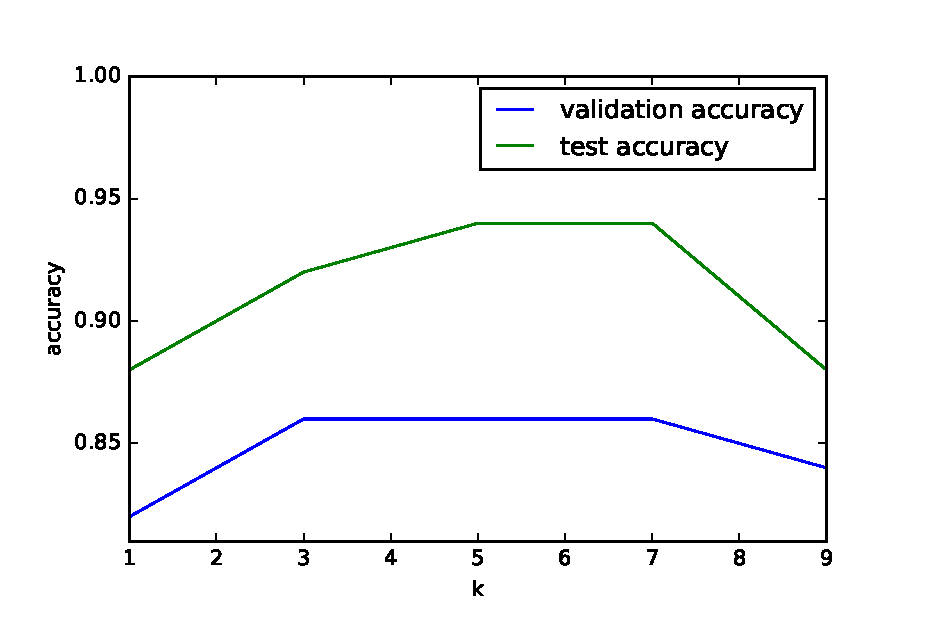
\includegraphics[scale=.65]{plot1.eps}
\caption{The Accuracy Plot against $k$}
\label{plot1}
\end{figure}
As we observe from the plot, the accuracies show incresing-then-decreasing trends on both validation set and test set as $k$ grows. The highest accuracies in validation set and test set are $0.86$ and $0.94$ respectively, when $k \in \{3, 5, 7\}$ and $k \in \{5, 7\}$.\par
The optimal $k$ I chose is $k^* = 5$, at which the validation accuracy and the test accuracy are $0.86$ and $0.94$ (both are peaks) respectively. The accuracies of $k^* - 2$ and $k^* + 2$ of the validation set are both $0.86$, and that of the test set are $0.92$ and $0.94$. I chose $k^* = 5$ because the performances on $k^* - 2$ and $k^* + 2$ are both efficient on both sets, which makes $k^*$ a relatively stable peak, and then it is more probable to perform more efficiently on other test sets.\par
The trends as $k$ grows in each set are similar, but the performance on the test set are much better than the validation set, probably because the data in test set is more similar to the training set than the data in validation set (splitting training data to training set and validation set unevenly may cause this problem).
\subsection{Logistic Regression}
Based on the model deduced in section \ref{subsec_mle}, we implemented the logistic regression on both \texttt{mnist\_train} and \texttt{mnist\_train\_small}.\par
\subsubsection{Hyperparameters Tuning}
Before testing the model, we need to tune the hyperparameters based on the training set and the validation set, in order to get the optimal model. There are three key hyperparameters to tune
\begin{itemize}
\item Learning rate: I have tried multiple values in $\{0.001, 0.01, 0.1, 1, 10, 100\}$ as the learning rate and observed that when it came to $100$, I got a \texttt{Nan} error, and when it came to $10$, the oscillation of the cross entropy is too strong. And when it came too little, the convergence speed is relatively low, thus the chosen learning rate would be $1$.
\item Iteration times: as the learning rate being fixed at $1$, the number iteration times when convergent is around $45$ on \texttt{mnist\_train} and $20$ on \texttt{mnist\_train\_small}, thus I set the iteration times to $50$ and $25$ respectively.
\item Weight initialization: I have tried multiple distributions (e.g. standard normal distribution, standard uniform distribution), and observed that the standard uniform distribution showed a better performance on accuracies, etc. Thus I chose the standard uniform distribution as the initial weight.
\end{itemize}
\subsubsection{Model Performance}
Fixing the hyperparameters and training the model, we have the final cross entropies and error rates as the follow tables show
\begin{table}[H]
\begin{minipage}{.5\linewidth}
\centering
\begin{tabular}{|c|c|c|c|}
\hline
 & train & valid & test\\
\hline
CE & $0.010785$ & $0.045450$ & $0.020982$ \\
\hline
Err & $0$ & $0.08$ & $0.06$ \\
\hline
\end{tabular}
\caption{Final Results on \texttt{mnist\_train}}
\end{minipage}
\ 
\begin{minipage}{.5\linewidth}
\centering
\begin{tabular}{|c|c|c|c|}
\hline
 & train & valid & test\\
\hline
CE & $0.001631$ & $0.041588$ & $0.017804$ \\
\hline
Err & $0$ & $0.32$ & $0.24$ \\
\hline
\end{tabular}
\caption{Final Results on \texttt{mnist\_train\_small}}
\end{minipage}
\end{table}
As we observe from the tables above, the final CE and error rates showed efficient performances on all the three sets on \texttt{mnist\_train}, and the test performance is better than the valid performance. However for \texttt{mnist\_train\_small}, the performance is limited by its small scale, and the test performance is also better than the valid performance.\par
The CE and accuracy plots against iteration times on both \texttt{mnist\_train} and \texttt{mnist\_train\_small} are shown as follows
\begin{figure}[H]
\centering
\begin{minipage}[b]{0.45\textwidth}
\centering
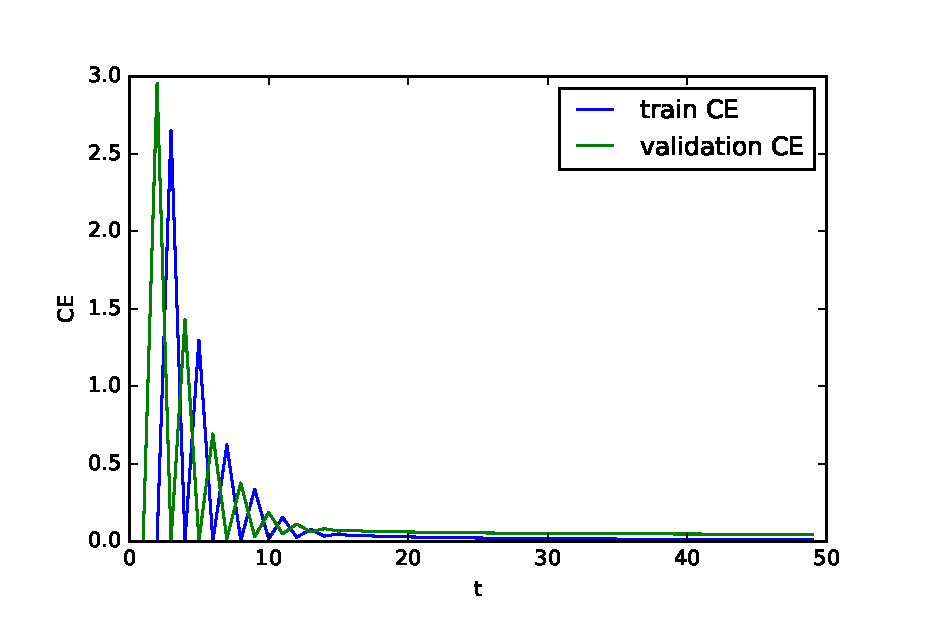
\includegraphics[scale=.5]{plot_big_ce.eps}
\caption{CE on \texttt{mnist\_train}}
\label{plot_big_ce}
\end{minipage}
\
\begin{minipage}[b]{0.45\textwidth}
\centering
\includegraphics[scale=.5]{plot_big_acc.eps}
\caption{Accuracies on \texttt{mnist\_train}}
\label{plot_big_acc}
\end{minipage}
\end{figure}
\begin{figure}[H]
\centering
\begin{minipage}[b]{0.45\textwidth}
\centering
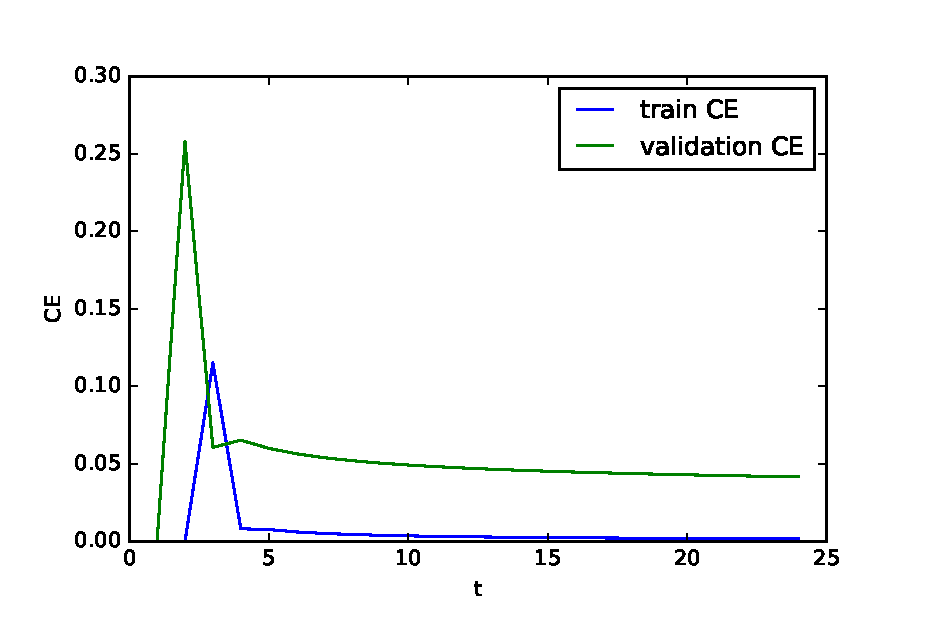
\includegraphics[scale=.5]{plot_small_ce.eps}
\caption{CE on \texttt{mnist\_train\_small}}
\label{plot_small_ce}
\end{minipage}
\
\begin{minipage}[b]{0.45\textwidth}
\centering
\includegraphics[scale=.5]{plot_small_acc.eps}
\caption{Accuracies on \texttt{mnist\_train\_small}}
\label{plot_small_acc}
\end{minipage}
\end{figure}
As we observe from the plots above, on \texttt{mnist\_train}, the CE showed a state of strong oscillation and decreasing in early iterations, and then the state declined, gradually showed a convergence state. However the oscillation state on \texttt{mnist\_train\_small} is much weaker, and its convergence state came earlier. The performances on the both dateset showed a great convergence speed.\par
Running my codes several times, the results changed just a little, probably because the randomness of the initial weights, and the sensitivity of the model to initial weights which may be determined by hyperparameters.\par
If the results changed a lot, I would tuning the parameters, for instance,
\begin{itemize}
\item Choosing a distribution of small range or small variance which generating the initial weights randomly.
\item Choosing a different model that is not as sensitive as before to the turbulance of initial weights.
\end{itemize}
\subsection{Penalized Logistic Regression}
Based on the model deduced in section \ref{subsec_l2}, and abandoning the bias term and the constant in $L\left(\mathbf{w}, b\right)$, we implemented the penalized logistic regression on both \texttt{mnist\_train} and \texttt{mnist\_train\_small}.
\subsubsection{Model Performance}
Tuning the $\lambda \in \{0.001, 0.01, 0.1, 1.0\}$, we have the average (through $10$ runs) CE and errors plots against $\log\lambda$ as follows
\begin{figure}[H]
\centering
\begin{minipage}[b]{0.45\textwidth}
\centering
\includegraphics[scale=.5]{plot_big_ce_pen.eps}
\caption{CE on \texttt{mnist\_train}}
\label{plot_big_ce_pen}
\end{minipage}
\
\begin{minipage}[b]{0.45\textwidth}
\centering
\includegraphics[scale=.5]{plot_big_err_pen.eps}
\caption{Errors on \texttt{mnist\_train}}
\label{plot_big_err_pen}
\end{minipage}
\end{figure}
\begin{figure}[H]
\centering
\begin{minipage}[b]{0.45\textwidth}
\centering
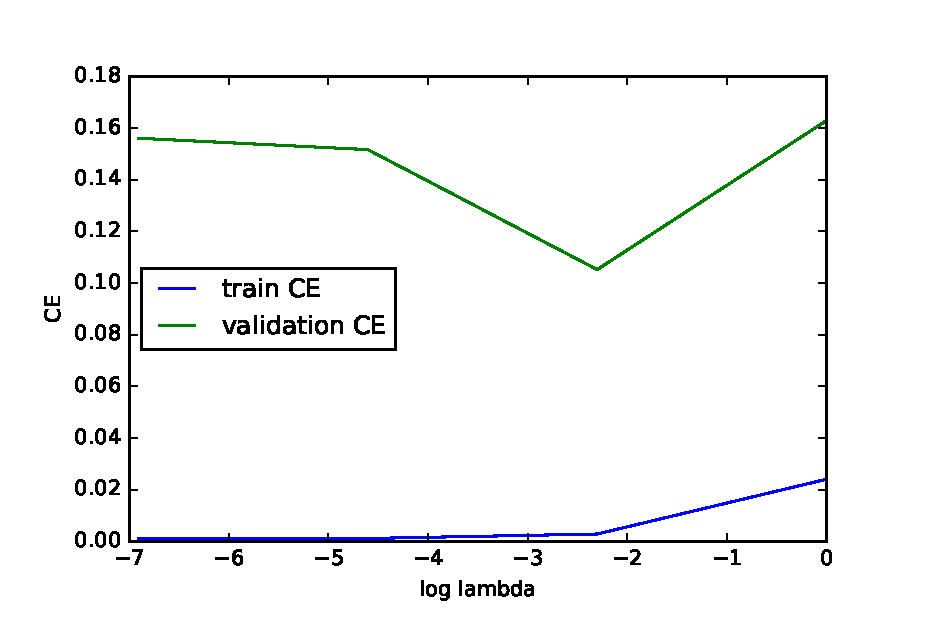
\includegraphics[scale=.5]{plot_small_ce_pen.eps}
\caption{CE on \texttt{mnist\_train\_small}}
\label{plot_small_ce_pen}
\end{minipage}
\
\begin{minipage}[b]{0.45\textwidth}
\centering
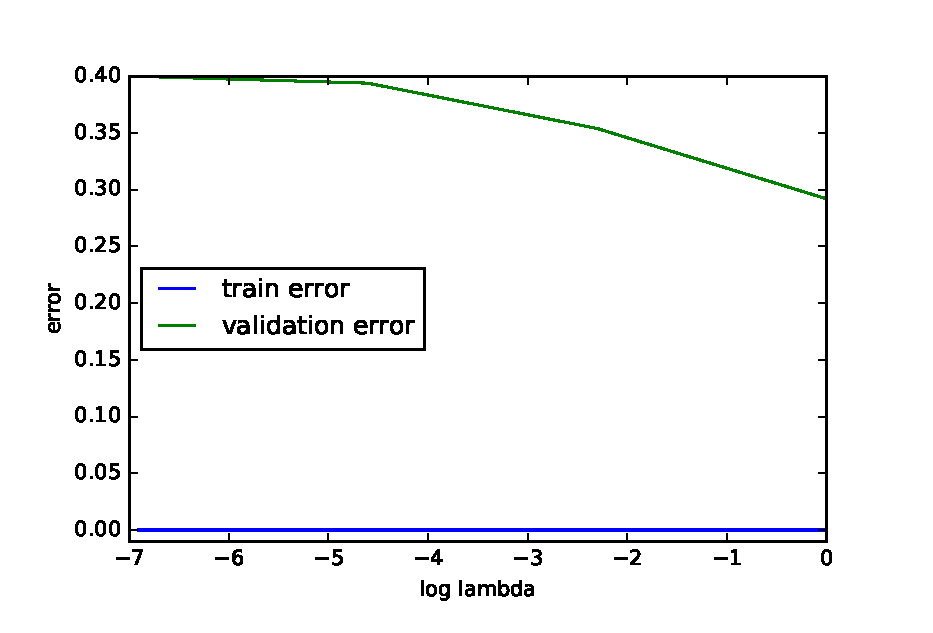
\includegraphics[scale=.5]{plot_small_err_pen.eps}
\caption{Errors on \texttt{mnist\_train\_small}}
\label{plot_small_err_pen}
\end{minipage}
\end{figure}
As we observe from the plots above, for \texttt{mnist\_train}, the train CE showed an increasing tread though all $\lambda$, however the validation CE went up, and then down, and then up, of which the optimal $\lambda$ with minimum validation CE is $\lambda = 0.1$, and the train error stayed at $0$, and the validation error had the same trend as CE, of which the optimum is also $\lambda = 0.1$. The valid CE and the valid error had the same trend probably because of the positive correlation between CE and error rate (generally speaking).\par
For \texttt{mnist\_train\_small}, the train CE showed an increasing tread though all $\lambda$, however the validation CE went up, and then down, of which the optimal $\lambda$ with minimum validation CE is $\lambda = 0.1$, and the train error stayed at $0$, however the validation error had a decreasing trend, of which the optimum is $\lambda = 1$. The valid CE and the valid error had different status when $\lambda = 1$, of which overfitting may be one of the reasons.\par
In general, the performances between $\lambda = 0.001$ and $\lambda = 0.01$ are close, which is probably because they are both too little to affect the training process. And if the regularization weight is large, it may weaken the minimization process of the true loss function, which may cause CE greater. Thus we take $\lambda = 0.1$ as the regularization parameter.\par
The test performance when $\lambda = 0.1$ on \texttt{mnist\_train} has a CE of $0.012254$ and an error rate of $0.06$. For \texttt{mnist\_train\_small}, the test performance has a CE of $0.050173$ and an error rate of $0.24$.\par
The test performance on \texttt{mnist\_train} is a little better when introducing penalty, however that on \texttt{mnist\_train\_small} is almost the same, even in the contrary. The reason may be that penalties on small datasets can affect the loss minimization negatively, and, that the dataset is so small that it has a greater uncertainty on performances. On large datasets with less uncertainty, penalties can prevent overfitting, which may probably improve the model performance.
\subsection{Naïve Bayes}
\subsubsection{Naïve Bayes Classifier}
Assuming that $\mathbf{x}$ is the feature vector (with $M = 784$ features) of an image and label $c = 0, 1$ represents $2$ classes respectively, the naïve bayes classifier can be written as
\begin{equation} \label{equ1}
\begin{aligned}
\Pr\left(c\mid \mathbf{x}\right) &= \dfrac{p\left(\mathbf{x} \mid c\right)\Pr\left(c\right)}{p\left(\mathbf{x}\right)} = \dfrac{p\left(\mathbf{x} \mid c\right)\Pr\left(c\right)}{p\left(\mathbf{x} \mid c = 0\right)\Pr\left(c = 0\right) + p\left(\mathbf{x} \mid c = 1\right)\Pr\left(c = 1\right)}\\
&\propto p\left(\mathbf{x} \mid c\right)\Pr\left(c\right) = \Pr\left(c\right)\prod\limits_{i = 1}^{M}p\left(x_i \mid c\right)
\end{aligned}
\end{equation}
where prior $\Pr\left(c\right)$ and $p\left(x_i \mid c\right)$ will be obtained by frequency calculation and ML on the training dataset.\par
Based on the maximum a posteriori estimation (in spite of the parameters in $p\left(x_i \mid c\right)$), the classifier can be written as
$$c_{\text{o}}(\mathbf{x}) = \argmax_{c}\Pr\left(c\right)\prod\limits_{i = 1}^{M}p\left(x_i \mid c\right),\, c = 0, 1\text{.}$$\par
For the ML of $p\left(x_i \mid c\right)$, the Gaussian distribution has a ML of
$$\hat{\mu} = \frac{\sum X_i}{N},\, \hat{\sigma}^2 = \frac{\sum\left(X_i - \hat{\mu}\right)^2}{N}\text{,}$$
hence
$$\hat{\mu}_{jc} = \frac{\sum\limits_{i = 1}^NX_{ij}\mathbbm{1}_{\{c\}}(c_i)}{\sum\limits_{i = 1}^N\mathbbm{1}_{\{c\}}(c_i)},\, \hat{\sigma}_{jc}^2 = \dfrac{\sum\limits_{i = 1}^N\left(X_i - \hat{\mu}_{jc}\right)^2\mathbbm{1}_{\{c\}}(c_i)}{\sum\limits_{i = 1}^N\mathbbm{1}_{\{c\}}(c_i)}\text{,}$$
where $\mathbbm{1}_{\{c\}}(c_i)$ is the indicator function.
\subsubsection{Model Performance}
After fitting the naïve Bayes model, the predictions has an accuracy of $0.8625$ on training set and $0.8$ on testing set. The image of the mean and variance vector $\boldsymbol{\mu}_c$ and $\boldsymbol{\sigma}_c^2$ for both models are shown as follows
\begin{figure}[H]
\centering
\begin{minipage}[b]{0.45\textwidth}
\centering
\includegraphics[scale=.5]{image_mean.eps}
\caption{The Mean Images of Both Classes}
\label{image_mean}
\end{minipage}
\
\begin{minipage}[b]{0.45\textwidth}
\centering
\includegraphics[scale=.5]{image_var.eps}
\caption{The Variance Images of Both Classes}
\label{image_var}
\end{minipage}
\end{figure}
As we observe from the images above, the $2$ classes are digit 4 and digit 9. In the mean images, the internal parts of the drawing lines of the digits are lighter than the contour lines, however the variance images is quite the opposite that the contour lines are much lighter. In other words, the mean image and the variance image are complementary in each class.\par
Based on the observation, we can infer that the internal parts of the drawing lines are lighter in mean images because the same digits are roughly in the same shapes, however the exact shapes are unstable, therefore the variances on the edges of the shapes are relatively greater.
\subsection{Comparison}
We have implemented $k$-NN, logistic regression (with or without penalty) and naïve Bayes model on \texttt{MNIST} data, and they have their own pros and cons
\begin{itemize}
\item $k$-NN \cite{keller1985fuzzy} does not actually have a training process, the model parameters are the training data itself, which costs plenty of storage. However its performance is efficient.
\item Logistic regression \cite{hosmer2013applied} has a training process which fit large dataset to model parameters, and it has many mutant formation (e.g. with penalty, with other loss functions). In this project, the loss function is negative log likelihood function.
\item Naïve Bayes \cite{mccallum1998comparison} is a classic statistic model, which fit the dataset to required probabilities or probability densities based on frequency.
\end{itemize}
The testing accuracies are shown as the following table below
\begin{center}
\begin{tabular}{|c|c|c|c|c|}
\hline
 & $k$-NN & LR & LR (with P) & NB\\
\hline
test & $0.94$ & $0.94$ & $0.94$ & $0.8$ \\
\hline
\end{tabular}
\end{center}
From the table we can conclude that $k$-NN, logistic regression (with or without penalty) has a efficient performance on \texttt{MNIST}, of which the testing accuracies are all $0.94$. The naïve Bayes model is much less efficient on testing performance, only $0.8$.
\section{Stochastic Subgradient Methods}
Considering the minimization of the SVM objective function
$$
\min_{\mathbf{w}}f\left(\mathbf{w}\right) = \dfrac\lambda2\norm{\mathbf{w}}^2 + \dfrac1n\sum\limits_{i=1}^n\max\left\{0, 1 - y_i\mathbf{w}^\intercal\mathbf{x}_i\right\}
$$
of whose $f\left(\mathbf{w}\right)$ the sub-gradient is
$$
\lambda\mathbf{w} + \begin{cases}
-y_i\mathbf{x}_i, &\, \text{if } 1 - y_i\left(\mathbf{w}^\intercal\mathbf{x}\right) > 0 \\
0, &\, \text{otherwise}
\end{cases} \in \partial f\left(\mathbf{w}\right)\text{,}
$$
thus the stochastic subgradient method would be
$$
\mathbf{w}^{t+1} = \mathbf{w}^t - \alpha_t\left(\lambda\mathbf{w}^t + \begin{cases}
-y_{i_t}\mathbf{x}_{i_t}, &\, \text{if } 1 - y_{i_t}\left({\mathbf{w}^t}^\intercal\mathbf{x}_{i_t}\right) > 0 \\
0, &\, \text{otherwise}
\end{cases}\right)
$$
\subsection{Polyak-Ruppert Averaging}
Define the running average $\bar{\mathbf{w}}^t = \sum\limits_{i=0}^{t-1}\mathbf{w}^i$, and replace the current $\mathbf{w}^t$ by $\bar{\mathbf{w}}^t$ in each performance testing step \cite{polyak1992acceleration}. The plot of the value of objective function against performance testing steps generated by \texttt{svmAvg} is shown as follows
\begin{figure}[H]
\centering
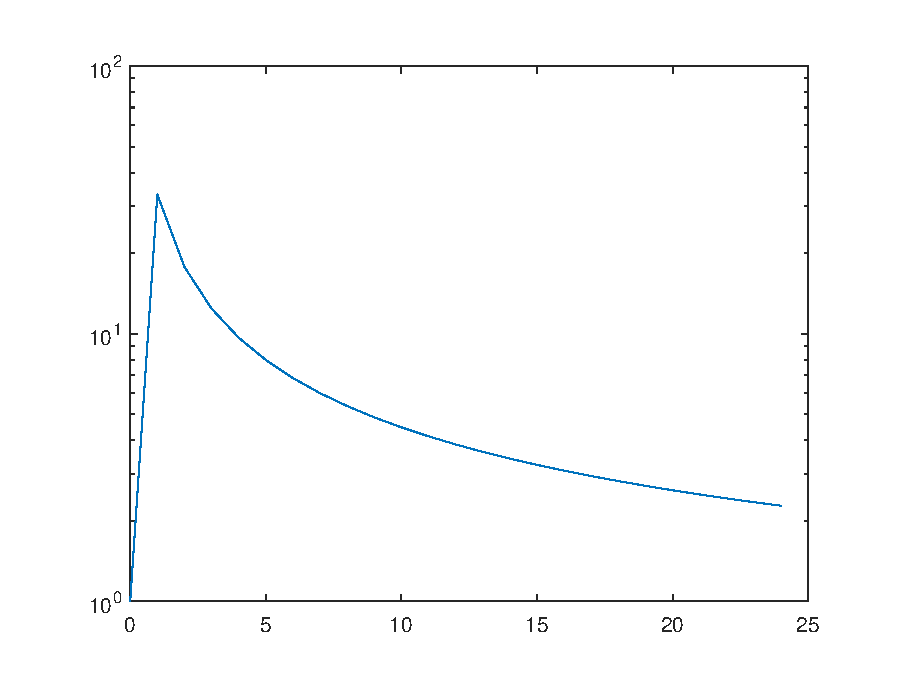
\includegraphics[scale=.65]{bonus1.eps}
\caption{The Function Value Plot}
\label{bonus1}
\end{figure}
As we observe from the plot, although averaging all the iterations smoothed the performance, the objective function was still increased compared to its initial value.\par
The modified part of the code is in appendix \ref{app_A}.
\subsection{Second-Half Averaging}
Define the second-half running average $\bar{\mathbf{w}}^t = \sum\limits_{i=\left\lceil\frac{maxIter}{2}\right\rceil}^{t-1}\mathbf{w}^i$, where $t > \left\lceil\frac{maxIter}{2}\right\rceil$. Remaining the first half of $\mathbf{w}^t$ where $t \leq \left\lceil\frac{maxIter}{2}\right\rceil$ and replacing the other half to $\bar{\mathbf{w}}^t = \sum\limits_{i=\left\lceil\frac{maxIter}{2}\right\rceil}^{t-1}\mathbf{w}^i$, we have the plot of the value of objective function against performance testing steps generated by modified \texttt{svmAvg}
\begin{figure}[H]
\centering
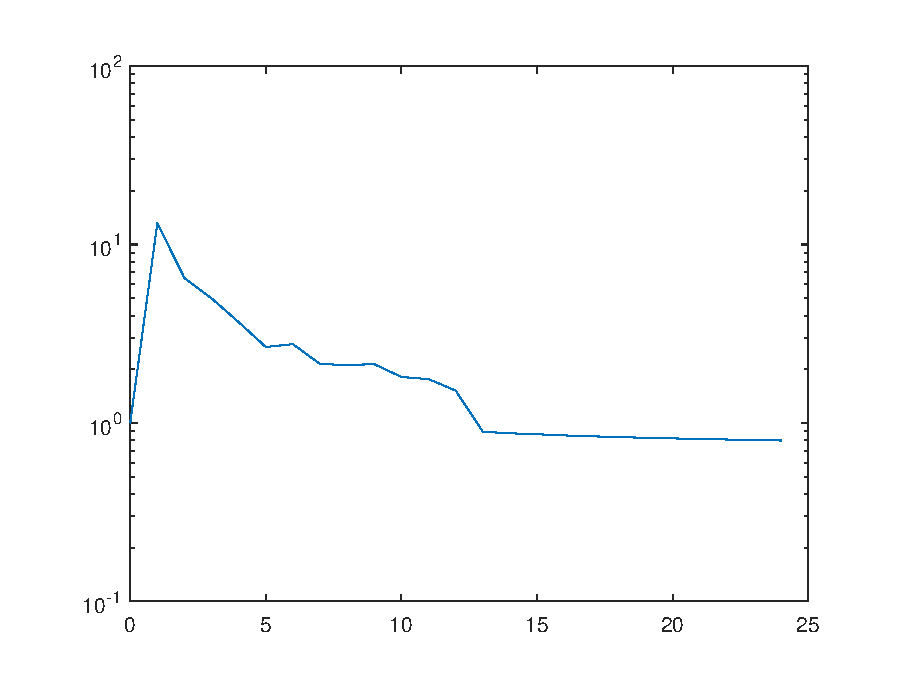
\includegraphics[scale=.65]{bonus2.eps}
\caption{The Function Value Plot}
\label{bonus2}
\end{figure}
As we observe from the plot, averaging the iterations of the second half smoothed the performance of the second half, the objective function value decreased to around $0.8$, in a convergence state.\par
The modified part of the code is in appendix \ref{app_A}.
\subsection{Additional Optimization}
I applied the modified SAG (Stochastic Average Gradient) method \cite{roux2012stochastic}
$$
\mathbf{w}^{t+1} = \mathbf{w}^t - \frac{\alpha_t}n\sum\limits_{i=1}^n\mathbf{g}_i^{t + 1}, \, \mathbf{g}_i^{t + 1} = \begin{cases}
\nabla f_i\left(\mathbf{w}^t\right),&\, i = i_t
\\
\mathbf{g}_i^{t},&\, i \neq i_t
\end{cases}
$$
with another initial condition $\mathbf{g}_i^{0} = \nabla f_i\left(\mathbf{w}^0\right)$. The main idea of this algorithm is to store the previously calculated gradients, along with the newly calculated stochastic gradient, taking the average of these gradients as the final gradient of the current step. The optimization plot is shown as follows
\begin{figure}[H]
\centering
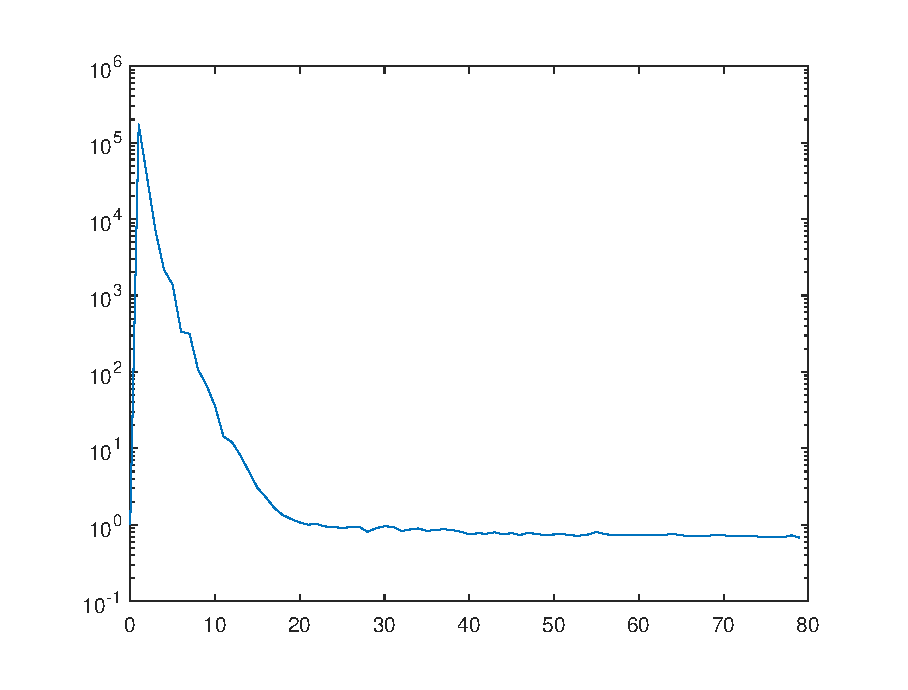
\includegraphics[scale=.65]{bonus3.eps}
\caption{The Function Value Plot (modified SAG)}
\label{bonus3}
\end{figure}
As we observe from the plot, in the early period of optimizing the function value reached beyond $10^5$. It has a fast down trend before the $20$-th iteration, and a slow down trend after. It has a faster convergence speed than averaging and a slower convergence speed than second-half averaging. However, the objective function value decreased to around $0.7$ in a convergence state, which is better than the previous methods.\par
The function \texttt{svmSAG} is in appendix \ref{app_A}.
\medskip
\bibliographystyle{plain}
\bibliography{ref}
\clearpage
\appendix
\section{MATLAB Codes for Stochastic Subgradient Methods}
\label{app_A}
Function \texttt{svmAvg} for averaging
\begin{lstlisting}[language=MATLAB]
function [model] = svmAvg(X, y, lambda, maxIter)

% Add bias variable
[n,d] = size(X);
X = [ones(n,1) X];

% Matlab indexes by columns,
%  so if we are accessing rows it will be faster to use  the traspose
Xt = X';

% Initial values of regression parameters
w = zeros(d + 1, 1);
w_set(:, 1) = w;

% Apply stochastic gradient method
for t = 1 : maxIter
  if mod(t - 1, n) == 0
    % Plot our progress
    % (turn this off for speed)
    w_mean = mean(w_set, 2);
    objValues(1 + (t - 1) / n) = (1 / n) * sum(max(0, 1 - y .* (X * w_mean))) + (lambda / 2) * (w_mean' * w_mean);
    semilogy([0 : t / n], objValues);
    pause(.1);
  end

  % Pick a random training example
  i = ceil(rand * n);

  % Compute sub-gradient
  [~, sg] = hingeLossSubGrad(w, Xt, y, lambda, i);

  % Set step size
  alpha = 1 / (lambda * t);

  % Take stochastic subgradient step
  w = w - alpha * (sg + lambda * w);
  w_set(:, t + 1) = w;
end

model.w = mean(w_set, 2);
model.predict = @predict;

end
\end{lstlisting}
\clearpage
Function \texttt{svmAvg} for second-half averaging
\begin{lstlisting}[language=MATLAB]
function [model] = svmAvg(X, y, lambda, maxIter)

% Add bias variable
[n,d] = size(X);
X = [ones(n,1) X];

% Matlab indexes by columns,
%  so if we are accessing rows it will be faster to use  the traspose
Xt = X';

% Initial values of regression parameters
w = zeros(d + 1, 1);
w_set = []
% Apply stochastic gradient method
for t = 1 : maxIter

    if t >= maxIter / 2
        w_set = [w_set, w];
    end

    if mod(t - 1, n) == 0
        % Plot our progress
        % (turn this off for speed)
        if t >= maxIter / 2
            w_ = mean(w_set, 2);
        else
            w_ = w
        end
        objValues(1 + (t - 1) / n) = (1 / n) * sum(max(0, 1 - y .* (X * w_))) + (lambda / 2) * (w_' * w_);
        semilogy([0 : t / n], objValues);
        pause(.1);
    end
    
    % Pick a random training example
    i = ceil(rand * n);
    
    % Compute sub-gradient
    [~, sg] = hingeLossSubGrad(w, Xt, y, lambda, i);
    
    % Set step size
    alpha = 1 / (lambda * t);
    
    % Take stochastic subgradient step
    w = w - alpha * (sg + lambda * w);
    
end

model.w = mean(w_set, 2);
model.predict = @predict;

end
\end{lstlisting}
\clearpage
Function \texttt{svmSAG} for modified SAG
\begin{lstlisting}[language=MATLAB]
function [model] = svmSAG(X, y, lambda, maxIter)

% Add bias variable
[n,d] = size(X);
X = [ones(n,1) X];

% Matlab indexes by columns,
%  so if we are accessing rows it will be faster to use  the traspose
Xt = X';

% Initial values of regression parameters
w = zeros(d + 1, 1);
gradient = zeros(d + 1, n);

for i = 1 : n
  [~, gradient(:, i)] = hingeLossSubGrad(w, Xt, y, lambda, i);
end

sum_gradient = sum(gradient, 2);

% Apply stochastic gradient method
for t = 1 : maxIter
  if mod(t - 1, n) == 0
    % Plot our progress
    % (turn this off for speed)
        
    objValues(1 + (t - 1) / n) = (1 / n) * sum(max(0, 1 - y .* (X * w))) + (lambda / 2) * (w' * w);
    semilogy([0 : t / n], objValues);
    pause(.1);
  end
    
  % Pick a random training example
  i = ceil(rand * n);

  % Compute sub-gradient
  [~, sg] = hingeLossSubGrad(w, Xt, y, lambda, i);

  sum_gradient = sum_gradient - gradient(:, i) + sg + lambda * w;
  gradient(:, i) = sg + lambda * w;

  % Set step size
  alpha = 1 / (lambda * t);
    
  % Take stochastic subgradient step
  w = w - (alpha / n) * sum_gradient;

end

model.w = w;
model.predict = @predict;

end
\end{lstlisting}
\end{document}